\documentclass[11pt,journal]{article}
%\usepackage{hyperref}
%\usepackage[breaklinks]{hyperref}
\usepackage{breakurl}
\usepackage{url}
\usepackage{listings}
\usepackage{courier}
\usepackage{amsmath}

\usepackage{graphicx}
\graphicspath{ {/home/agata/Documents/coursework/NLP/exercise1/} }
%\ifCLASSOPTIONcompsoc
% IEEE Computer Society needs nocompress option
% requires cite.sty v4.0 or later (November 2003)
\usepackage[nocompress]{cite}

%\else
% normal IEEE
\usepackage{cite}
%\fi

\hyphenation{op-tical net-works semi-conduc-tor}
\addtolength{\oddsidemargin}{-.875in}
\addtolength{\evensidemargin}{-.875in} 
\addtolength{\textwidth}{1.75in}

\addtolength{\topmargin}{-.875in}
\addtolength{\textheight}{1.75in}

\begin{document}
	\title{CS909: Natural Language Processing, Exercise 1}
	
	\author{UID: 1690550}% <-this % stops a space
		%\protect\\
		%\thanks{}}
	
	% The paper headers



	% IEEEtran.cls defaults to using nonbold math in the Abstract.
	% This preserves the distinction between vectors and scalars. However,
	% if the journal you are submitting to favors bold math in the abstract,
	% then you can use LaTeX's standard command \boldmath at the very start
	% of the abstract to achieve this. Many IEEE journals frown on math
	% in the abstract anyway. In particular, the Computer Society does
	% not want either math or citations to appear in the abstract.
	
	% Note that keywords are not normally used for peerreview papers.
	
	% make the title area
	\maketitle
	
	
	% To allow for easy dual compilation without having to reenter the
	% abstract/keywords data, the \IEEEcompsoctitleabstractindextext text will
	% not be used in maketitle, but will appear (i.e., to be "transported")
	% here as \IEEEdisplaynotcompsoctitleabstractindextext when compsoc mode
	% is not selected <OR> if conference mode is selected - because compsoc
	% conference papers position the abstract like regular (non-compsoc)
	% papers do!
	%\IEEEdisplaynotcompsoctitleabstractindextext
	% \IEEEdisplaynotcompsoctitleabstractindextext has no effect when using
	% compsoc under a non-conference mode.
	
	
	% For peer review papers, you can put extra information on the cover
	% page as needed:
	% \ifCLASSOPTIONpeerreview
	% \begin{center} \bfseries EDICS Category: 3-BBND \end{center}
	% \fi
	%
	% For peerreview papers, this IEEEtran command inserts a page break and
	% creates the second title. It will be ignored for other modes.
	%\IEEEpeerreviewmaketitle
	\section{Part B}
	Operation costs:
	\begin{itemize}
		\item insertion: 1
		\item deletion: 1
		\item substitution: 2
	\end{itemize}
	\subsection{Minimum edit distance from "refa" to "fear"}
	\begin{table}[h]
		\centering
		\begin{tabular}{c|c c c c c}
			& \# & f & e & a & r \\
			\hline
			\# & 0 & 1 & 2 & 3 & 4 \\
			r & 1 & 2 & 3 & 4 & 3 \\
			e & 2 & 3 & 2 & 3 & 4 \\
			f & 3 & 2 & 3 & 4 & 5 \\
			a & 4 & 3 & 4 & 3 & 4 \\
		\end{tabular}
		\caption{Minimum edit distance of "refa" to "fear" is \underline{4}.}
	\end{table}

	There are 2 alignments, discovered by inspection. The alignments are:
	
	\begin{table}[h]
		\centering
		\begin{tabular}{c c c c c c}
			* & * & f & e & a & r \\
			$\vert$ & $\vert$ & $\vert$ & $\vert$ & $\vert$ & $\vert$ \\
			r & e & f & * & a & * \\
		\end{tabular}
	\end{table}
	
	
		\begin{table}[h]
		\centering
		\begin{tabular}{c c c c c c}
			* & f & e & * & a & r \\
			$\vert$ & $\vert$ & $\vert$ & $\vert$ & $\vert$ & $\vert$ \\
			r & * & e & f & a & *  \\
		\end{tabular}
	\end{table}

	\subsection{Minimum edit distance of "drive" to "brief and "drive" to "divers"}
	\begin{table}[h]
		\centering
		\begin{tabular}{c|c c c c c c}
			& \# & b & r & i & e & f \\
			\hline
			\# & 0 & 1 & 2 & 3 & 4 & 5\\
			 d & 1 & 2 & 3 & 4 & 5 & 6\\
			 r & 2 & 3 & 2 & 3 & 4 & 5\\
			 i & 3 & 4 & 3 & 2 & 3 & 4\\
			 v & 4 & 5 & 4 & 3 & 4 & 5\\
			 e & 5 & 6 & 5 & 4 & 3 & 4\\
			
		\end{tabular}
		\caption{Minimum edit distance of "drive" to "brief" is 4}
	\end{table}
	
	\begin{table}[h]
		\centering
		\begin{tabular}{c|c c c c c c c}
			& \# & d & i & v & e & r & s \\
			\hline
			\# & 0 & 1 & 2 & 3 & 4 & 5 & 6\\
			 d & 1 & 0 & 1 & 2 & 3 & 4 & 5\\
			 r & 2 & 1 & 2 & 3 & 4 & 3 & 4\\
			 i & 3 & 2 & 1 & 2 & 3 & 4 & 5\\
			 v & 4 & 3 & 2 & 1 & 2 & 3 & 4\\
			 e & 5 & 4 & 3 & 2 & 1 & 2 & 3\\
			
		\end{tabular}
		\caption{Minimum edit distance of "drive" to "divers" is 3}
	\end{table}
\pagebreak
	\section{Part C}
	
	For the purpose of this problem, we define the following sets:
	\[vowel = \{a,e,o,u,i\}\]
	\[consonant = \Sigma - vowel\]
	The set of consonants will be abbreviated to "cons.".
	
	We are interested in an FST for the consonant doubling rule for verbs. It is important to stress that the FSTs presented below work only for regular verbs. 
	
	If the input is given on the lexical level, we can turn it into intermediate with the following FST:
	
	\begin{figure}[h]
		\centering
		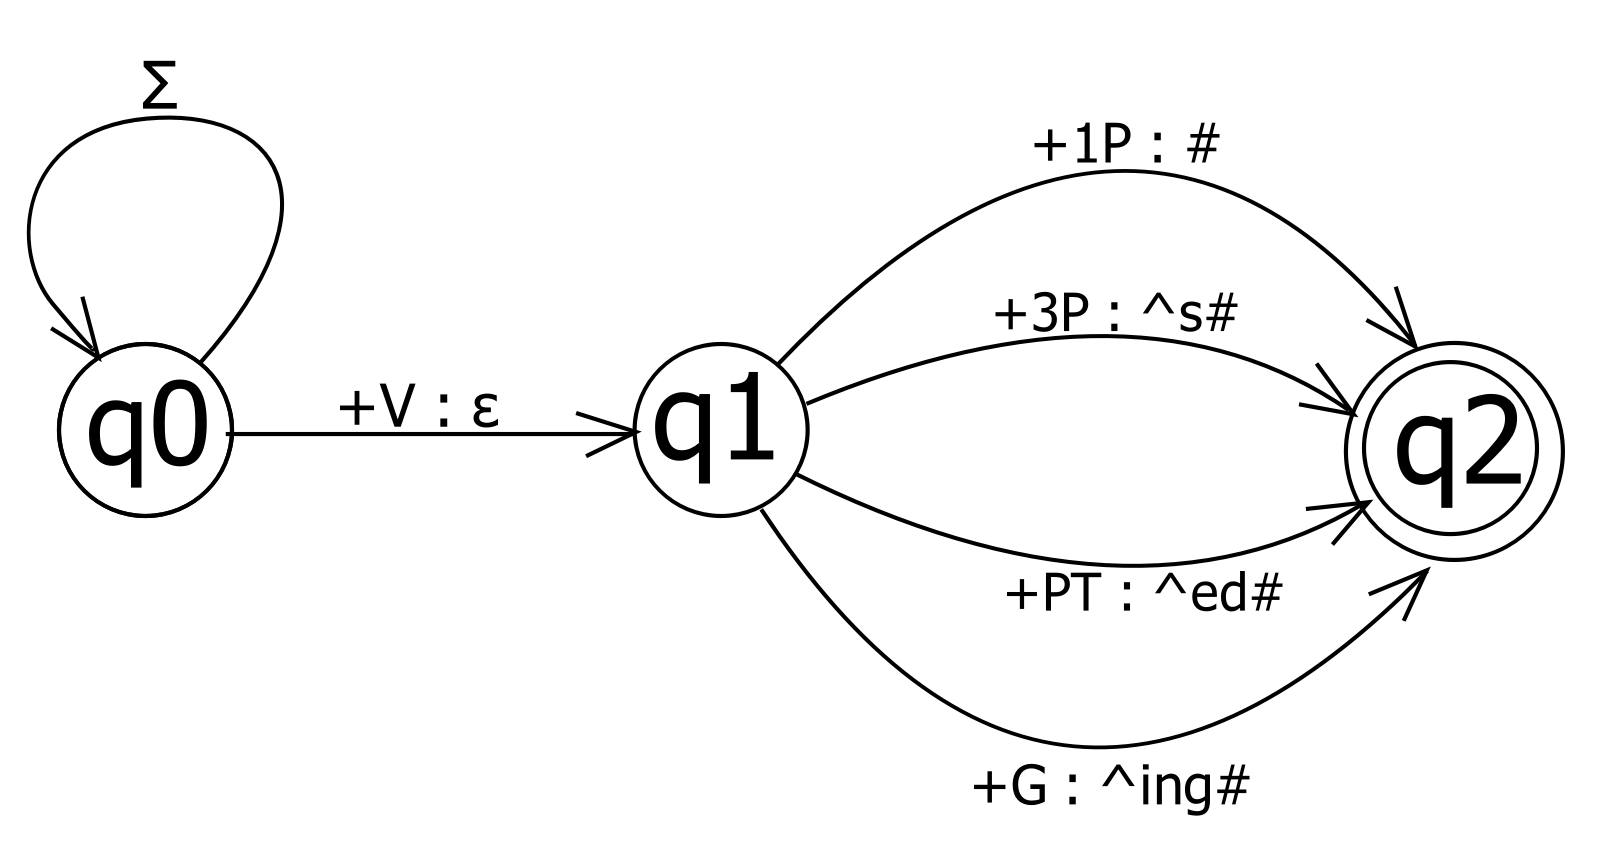
\includegraphics[]{fsa3.png}
		\caption{FST between lexical and intermediate level}
	\end{figure}

	Where $\Sigma$ is any letter, '+1P' indicates first person ending (same as stem), '+3P' indicates third person form (i.e. -s suffix), '+PT' stands for past tense (-ed), and '+G' for gerund (-ing).
	
	
	Figure 2 shows the simplest FST that encodes the consonant doubling rule just that for single syllable verbs, taking intermediate level input.  
	
	\begin{figure}[h]
		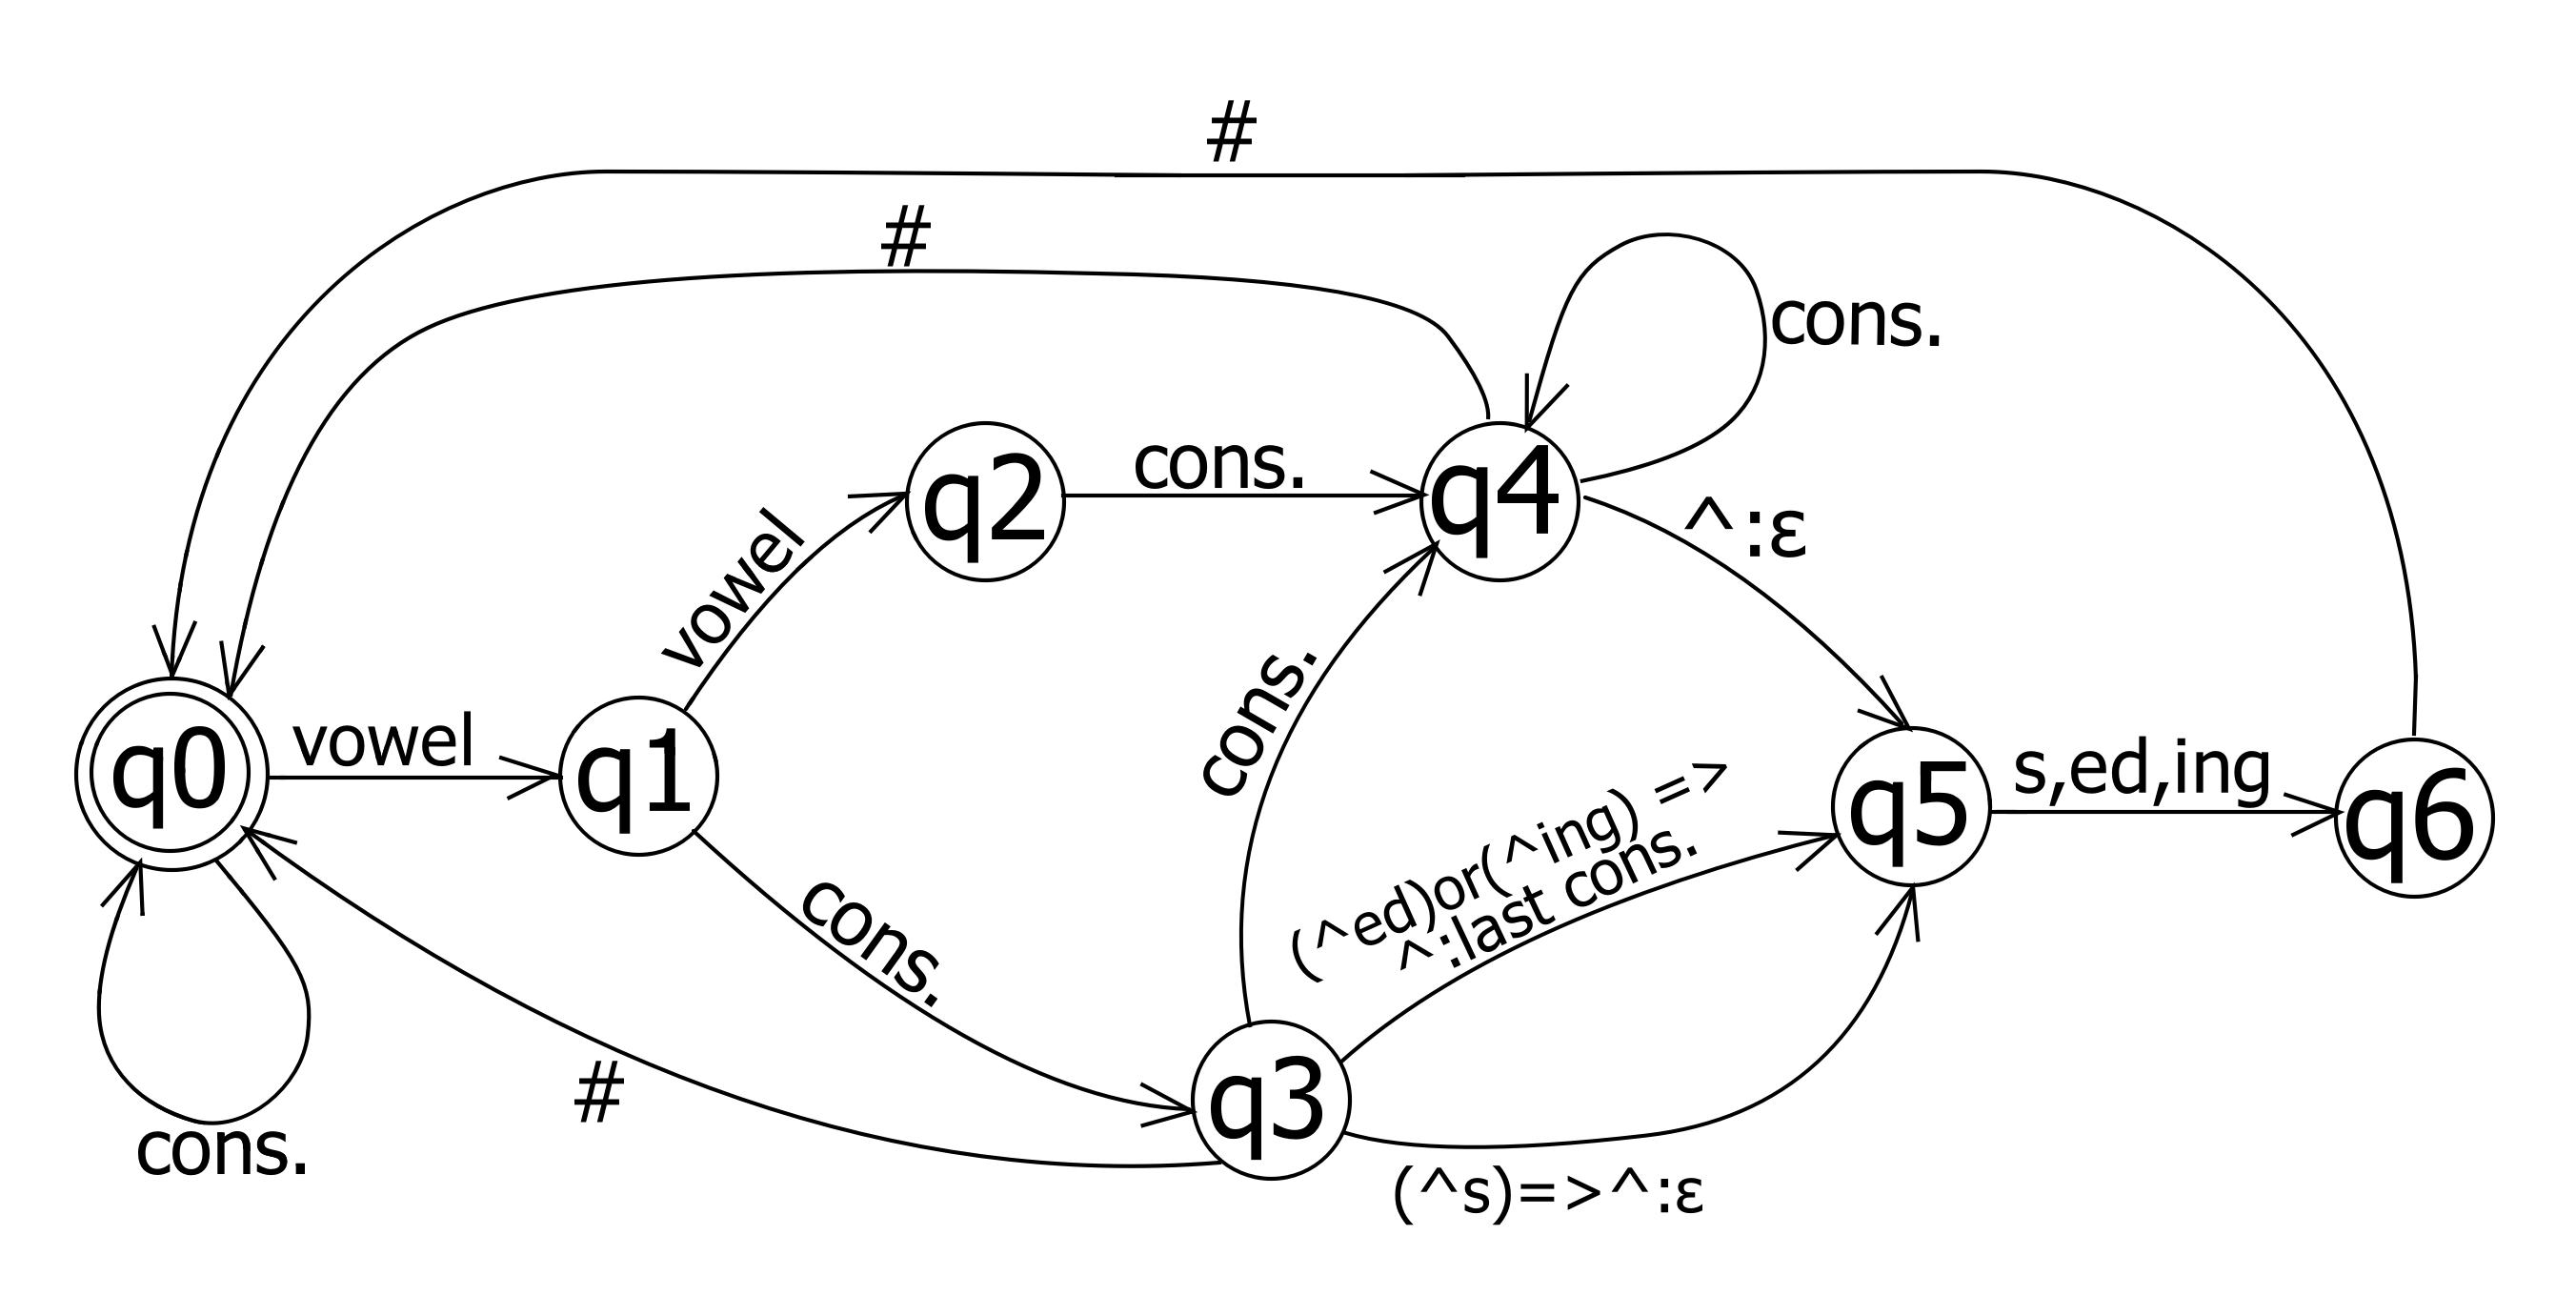
\includegraphics[scale=0.7]{fsa2.png}
		\caption{Simple version of the requested FST}
	\end{figure}

	The last consonant of the given verb will be doubled only if it is preceded by a single vowel, and if we are aiming for the regular past tense or the gerund of the verb.
	
	Thus for example:
	
	\begin{itemize}
		\item "aim" will go from state $q_0$ to $q_1$, then as we are seeing a second vowel, we go to $q_4$, and then either we see the end of the string symbol and go to the accepting state $q_0$, or add a required suffix.
		\item "bring" will loop over the "cons." edge around $q_0$ twice, then go to $q_1$ and on to $q_3$. Then, since we're seeing another consonant, we move to $q_4$ and avoid doubling the last letter.
		\item "stop" or "fit" will loop around $q_0$ until they get to $q_1$ and $q_3$. If the next character is the end of string symbol, we move back to the accepting state $q_0$. Otherwise, we read ahead to see what ending we need. If it's "s", we replace "$\wedge$" with empty symbol. Otherwise, we replace it with the last consonant.
	\end{itemize}

	However, this FST does not treat "e" at the end of the words correctly. Therefore we present a more robust version, which works for regular verbs, including those with multiple syllables and those ending in e (silent or otherwise).
	
	\begin{figure}[h]
		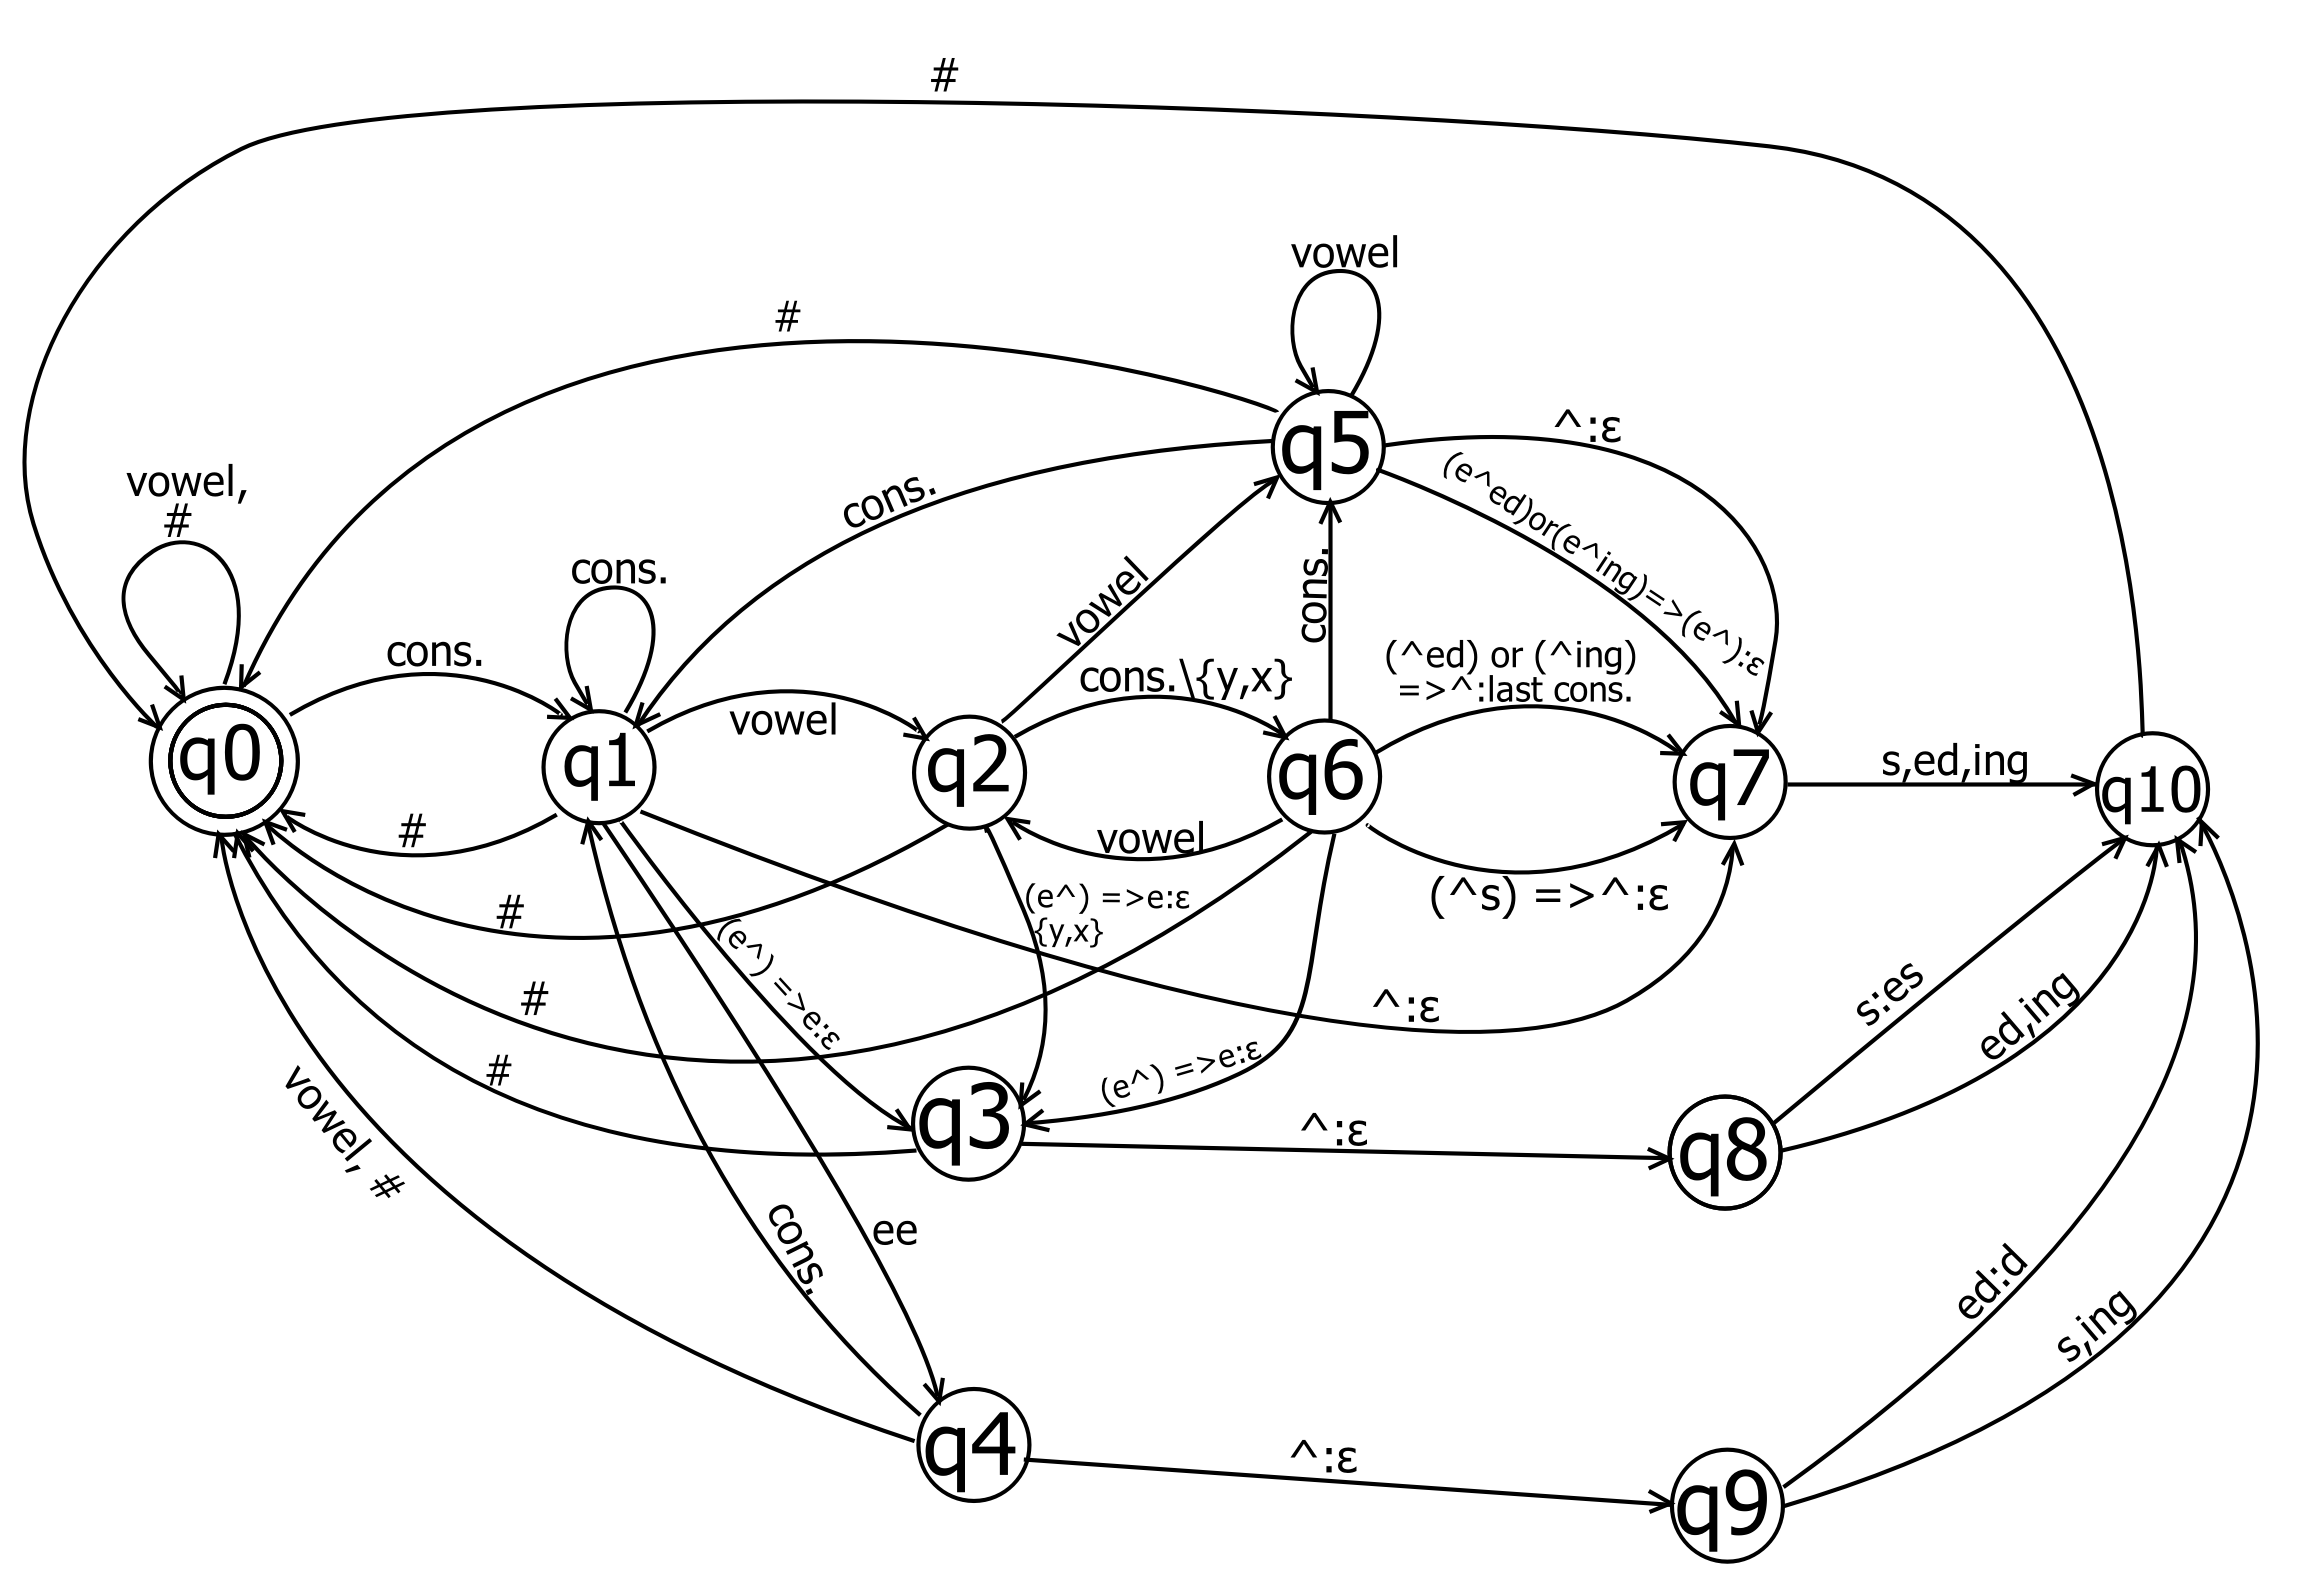
\includegraphics[scale=0.9]{fsa1.png}
		\caption{More robust FST}
	\end{figure}

	It is perhaps surprising that only states directly concerned with the consonants doubling are $q_0$, $q_1$, $q_2$, $q_6$, $q_7$, and $q_{10}$. The state $q_5$ is also important, as together with $q_1$ and $q_2$ it helps with detecting the 'consonant - vowel - consonant - $\wedge$' pattern. The rest deals with rules regarding e at the end of words.
	
	To explain what it does at each step, we shall inspect all outgoing edges from each node.
	
	\begin{itemize}
		\item $q_0$: we are coming back to it until we see the first consonant in the verb. Then we move to $q_1$
		
		\item $q_1$: this is the state from which be begin counting the consonants. I.e. we get to it after following a consonant. If we then see a vowel and a consonant, we apply the doubling rule. Other options are: double e (in words such as "agree") or a silent e where we focus on dealing with the rules regarding this, or "$\wedge$".
		
		\item $q_2$: the last consonant in a word here will get doubled, and so we proceed to $q_6$. However, the exceptions to this rule are the letters x and y. In these cases as well as a word-ending e (e.g. in "woe") we move to $q_3$. The last option is any vowel, leading to $q_5$.
		
		\item $q_3$: this is the state which catches "e $\wedge$" at the end of the stem. Note that we cannot get to $q_3$ without seeing $\wedge$, so we do not need an outgoing edge marked with end of string \# character.
		
		\item $q_4$: we treat double e separately, because in the case of past tense we lose the e in the suffix, but otherwise we don't alter the stem. There is a  very subtle difference between states $q_8$ and $q_9$ which we will analyse later. Words such as "agree" or "need" will go through this state.
	
		\item $q_5$: this state is part of the cycle detecting 'consonant - vowel - consonant' pattern. It will also detect the technically regular but difficult words such as "queue".\footnote{It is very likely that some simplifications can be made around this state}
		
		\item $q_6$: We can only get to this state after seeing the desired "consonant - vowel - consonant" pattern, and indeed all the incoming edges are from vowels. The two most important outgoing edges describe the consonant doubling rule and lead to $q_7$. The others are useful for when we have not reached the end of the word after spotting the pattern.
		
		\item $q_7$, $q_8$, and $q_9$ all deal with adding the desired suffix. In the first case, we take care of verbs ending with consonants (doubled or not). The latter two deal with words ending with e. Most of the words ending with a silent e will end up in $q_8$. To simplify dealing with it, we have removed the silent e, and so we can simply append the '-ed' and '-ing' suffixes. For the '-s' suffix, we need to add the e back again. $q_9$ is concerned with words ending in double e, such as 'agree' or 'free'. In these cases we did not remove any of the e's previously, and we can simply append '-ing' and '-s', but '-ed' gets shortened to just '-d'.
		
		\item Finally $q_{10}$ is reached after appending the desired suffix, and the only character we expect to see here is the end of string character, so we send the input to the accepting state $q_0$.
	
	\end{itemize}

	Here are some example of words accepted by this FST:
	\begin{itemize}
		\item "aim\#" (aim): $q_0 \rightarrow q_0 \rightarrow q_0 \rightarrow q_1 \rightarrow q_0$
		
		\item "aim$\wedge$ing\#" (aiming): $q_0 \rightarrow q_0\rightarrow q_0 \rightarrow  q_1 \rightarrow q_7 \rightarrow q_{10} \rightarrow q_0$
		
		\item "stop$\wedge$s\#" (stops): $q_0 \rightarrow q_1 \rightarrow q_1\rightarrow  q_2 \rightarrow  q_6 \rightarrow  \text{(following the bottom edge, no doubling) } q_7\rightarrow  q_{10} \rightarrow  q_0$
		
		\item "stop$\wedge$ed\#" (stopped): $q_0 \rightarrow q_1 \rightarrow  q_1 \rightarrow q_2 \rightarrow q_6 \rightarrow  \text{(following the top edge, doubling) } q_7\rightarrow  q_{10} \rightarrow  q_0$
		
		\item "free$\wedge$ed\#" (freed): $q_0\rightarrow q_1 \rightarrow  q_1 \rightarrow q_4 \rightarrow  q_9 \rightarrow \text{(following the top edge, to avoid triple e) } q_{10} \rightarrow  q_0$
		
		\item "like$\wedge$ing\#" (liking): $q_0 \rightarrow q_1 \rightarrow q_2\rightarrow q_6 \rightarrow  q_3 \rightarrow q_8 \rightarrow  \text{(following the bottom edge) } \rightarrow q_{10} \rightarrow  q_0$
		
		\item "queue$\wedge$ed\#" (queued): $q_0 \rightarrow q_1 \rightarrow q_2 \rightarrow q_5 \rightarrow q_5 \rightarrow q_7 \rightarrow q_{10} \rightarrow q_0$
	\end{itemize}
	
	
	%\IEEEPARstart{}{} 
	

	
	% that's all folks
\end{document}

